\chapter{Análisis y diseño del sistema}

En este capítulo se expone el análisis de requisitos funcionales, la arquitectura software, la base de datos y la interfaz del usuario.

\section{Requisitos del sistema}
\label{section-requisitos}

Seguidamente (véase tabla \ref{tab:RF}) se presentan, en modo de tabla, los principales requisitos del sistema. Para su formulación se ha partido de los detalles incluidos en la sección 1.2 y se ha trabajado directamente con la empresa.

% Tabla con los requisitos del sistema

% \begin{table}[!h]
% \centering
% \begin{tabular}{|p{1cm}|p{14cm}|}
\begin{longtable}{|p{1cm}|p{14cm}|}
	\hline
	\textbf{ID} & \textbf{Requisito} \\
	\hline
	RF-1 	& 	Un usuario iniciará sesión en el sistema utilizando un identificador de usuario (nickname), contraseña y puesto. \\
	\hline
	RF-2	&	Un usuario verá como opciones del campo puesto en la autenticación, las existentes en los recursos de ese tipo de la base de datos. En caso de que no exista ningún recurso de ese tipo, verá la opción "Puesto único".	\\
	\hline
	RF-3	&	Un usuario podrá cerrar su sesión.	\\
	\hline
	RF-4	&	El sistema permitirá al usuario navegar en la aplicación mediante un menú lateral. \\
	\hline
	RF-5	&	El sistema mostrará al usuario un listado de plantas del edificio. \\
	\hline
	RF-6	&	El sistema mostrará alertas de dos tipos al usuario: alarmas y presencias activas. \\
	\hline
	RF-7	&	Las alarmas son generadas por los pacientes en una situación de emergencia desde un terminal. Son de uno de los tipos que se encuentran en la base de datos. Se muestran si se encuentran en cualquiera de los tres estados explicados en la \hyperref[section-objetivos]{sección 1.2}. Los colores de estas alarmas según su estado son: rojo si está disparada; amarilla si está aceptada; y azul si está atendida. \\
	\hline
	RF-8	&	Las presencias activas son presencias de un trabajador en una habitación y pueden ser los dos tipos explicados en la \hyperref[section-objetivos]{sección 1.2}. \\
	\hline
	RF-9	&	El sistema mostrará al usuario el número total de alarmas y presencias activas en cada planta. \\
	\hline
	RF-10	&	El sistema permitirá al usuario elegir una planta y ver la información de las alertas correspondiente a esa planta. \\
	\hline
	RF-11	&	El sistema mostrará al usuario un carrusel (presentación de tarjetas que se pueden recorrer de izquierda a derecha) con las alertas de la planta seleccionada. \\
	\hline
	RF-12	&	El usuario podrá ver las alertas más actuales en las primeras posiciones (izquierda) del carrusel. \\
	\hline
	RF-13	&	El sistema mostrará al usuario la información del paciente de las alarmas activas y el lugar y momento en el que se han disparado. \\
	\hline
	RF-14	&	El sistema mostrará al usuario la información del trabajador de las presencias activas identificadas y el lugar y momento en el que se han producido. \\
	\hline
	RF-15	&	El sistema mostrará al usuario el plano (imagen guardada en la base de datos) de la planta seleccionada.  \\
	\hline
	RF-16	&	El sistema destacará al usuario en el plano las alertas activas en cada habitación coloreando la habitación según el tipo de alerta, y en caso de ser alarma también según su estado, siguiendo la siguiente prioridad:
	\begin{enumerate}
		\item Rojo: alerta de tipo alarma y estado disparada
		\item Amarillo: alerta de tipo alarma y estado aceptada
		\item Azul: alerta de tipo alarma y estado atendida
		\item Verde: alerta de tipo presencia
	\end{enumerate}\\
	\hline
	RF-18	&	El sistema mostrará al usuario un icono en la habitación según la prioridad. \\
	\hline
	RF-19	&	El sistema permitirá clicar en los iconos para ver una tarjeta emergente con la información concreta de la alerta con mayor prioridad de las que se encuentran en el carrusel. \\
	\hline
	RF-20	&	El sistema mostrará al usuario el listado de alarmas pendientes con su información, sin filtrado por planta, e indicando además el tipo de alarma. \\
	\hline
	RF-21	&	El sistema mostrará al usuario el número total de alarmas y presencias de la institución. \\
	\hline
\caption{Requisitos funcionales del sistema}
\label{tab:RF}
\end{longtable}
	% \end{tabular}
% \end{table}

Los requisitos no funcionales definen los atributos de calidad del sistema describiendo de qué manera opera el sistema. Se presentan a coninuación (véase tabla \ref{tab:RNF}).

\begin{longtable}{|p{1,2cm}|p{13,8cm}|}
	\hline
	\textbf{ID} & \textbf{Requisito} \\
	\hline
	RNF-1 	& 	Será necesario disponer de conexión a la LAN en la que esté instalada el sistema. \\
	\hline
	RNF-2	&	El sistema estará disponible siempre y cuando el PAServidor y los servicios implicados estén activos. (Veáse la explicación de la arquitectura en la \hyperref[section-arquitectura]{sección 2.2}).	\\
	\hline
	RNF-3	&	El sistema será escalable y elástico para adaptarse a los diferentes tamaños de edificios, y por tanto al número de alertas activas, según la institución en la que se instale el sistema.\\
	\hline
	RNF-4	&	La conexión se realizará mediante websockets.\\
	\hline
	RNF-5	&	La aplicación web será capaz de reconectarse si pierde comunicación con el servicio.\\
	\hline
	RNF-6	&	El sistema está disponible para todos los navegadores más populares en sus versiones actualizadas.\\
	\hline
	RNF-7	&	Las contraseñas utilizadas en la autenticación se comparan con el PIN identificativo del trabajador en la base de datos. \\
	\hline
\caption{Requisitos no funcionales del sistema}
\label{tab:RNF}
\end{longtable}


\section{Arquitectura software del sistema}
\label{section-arquitectura}
% Explicar la arquitectura final del sistema

El despliegue del sistema se realizará en una red de área local (LAN) ya que tiene que servir para una institución sanitaria o socio-sanitaria en la que se instalará el sistema configurando la base de datos correspondiente a la información de dicha institución.\\

Para ver las relaciones entre el software y su entorno se utiliza una vista de distribución estilo despliegue. (Veáse la \textit{Figura 2.1}). \\

\begin{figure}[!h]
    \centering
    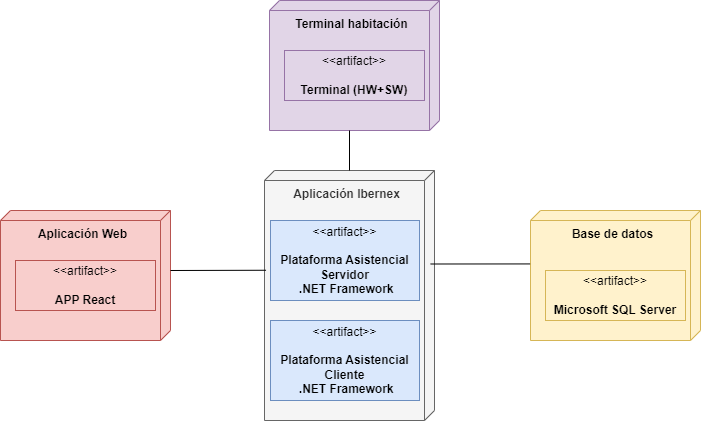
\includegraphics[width=15cm]{Imagenes/Arquitectura-despliegue}
    \caption{Diagrama de despliegue}
    \label{fig:despliegue}
\end{figure}

Con este diagrama se observan los elementos que han estado implicados en el proyecto. No obstante, lo que se ha implementado ha sido: la aplicación web completa y la funcionalidad añadida a la Plataforma Asistencial Servidor de la aplicación de Ibernex. A continuación se describen los elementos con mayor detalle:

\begin{itemize}
	\item \textbf{Plataforma Asistencial Servidor (PAServidor)} es la aplicación servidor del sistema asistencial Helpnex. Se trata de una aplicación monolítica modular. Dos de los elementos que componen la arquitectura de la aplicación son:
	\begin{itemize}
		\item Servicios: contienen la lógica del sistema Helpnex. Los servicios se cargan al inicio de la aplicación en función de la licencia adquirida. Cada servicio es el encargado de realizar una tarea específica. Algunos ejemplos de tareas son: comunicación con los terminales de habitación; gestionar las alarmas del sistema; comunicación con la aplicación web de monitorización; localización en interiores; comunicaciones SIP; entre otras.
		\item Cola de eventos: es el mecanismo de comunicación que utilizan los servicios para transmitir información entre ellos. Cada servicio se suscribe a una serie de eventos.
	\end{itemize}
	\item La \textbf{base de datos} es la que permite realizar la persistencia de datos de PAServidor, PACliente, la institución, los pacientes y resto de datos necesarios.
	\item La \textbf{aplicación web} que recibe los datos necesarios a monitorizar desde el nuevo servicio añadido a PAServidor para mostrarlos.
	\item \textbf{Plataforma Asistencial Cliente (PACliente)} es la encargada de gestionar la información del sistema Helpnex y guardarla en la Base de Datos. Se comunica con el PAServidor mediante una conexión socket TCP. La información se utiliza por PAServidor para realizar las gestiones necesarias. De igual forma, se compone de módulos que se gestionan mediante una licencia y permiten gestionar distintos elementos. Uno de los módulos sirve para configurar un sistema de reglas de notificación ante una alarma y esto es lo que permite al sistema generar las reglas y notificar por puestos la información que debe ser mostrada en la aplicación web.\\
	PACliente se ha utilizado en el proyecto  para realizar la gestión de plantas, habitaciones, residentes, terminales, trabajadadores, recursos de los puestos y configuración de reglas, teniendo una institución ficticia generada con datos de prueba durante todo el desarrollo.
	\item El \textbf{terminal} es el hardware que se encuentra en la habitación. En este contexto sirve tanto para notificar y codificar las alarmas como para registrar las presencias de trabajadores en las habitaciones. Existen otras tareas adicionales que pueden ser realizadas, pero que no están directamente relacionadas con el alcance de este proyecto.
\end{itemize}

% Hacer referencia al Anexo donde se expliquen las alternativas que se plantearon
La arquitectura aquí expuesta es la elegida entre las distintas opciones barajadas. Estas otras se pueden consultar con detalle en el \hyperref[anexo-a]{Anexo A}.\\

% Arquitectura del PAServidor
Para entender mejor la arquitectura del PAServidor se proporciona un diagrama más detallado. (Veáse la \textit{Figura 2.2}).

\begin{figure}[H]
    \centering
    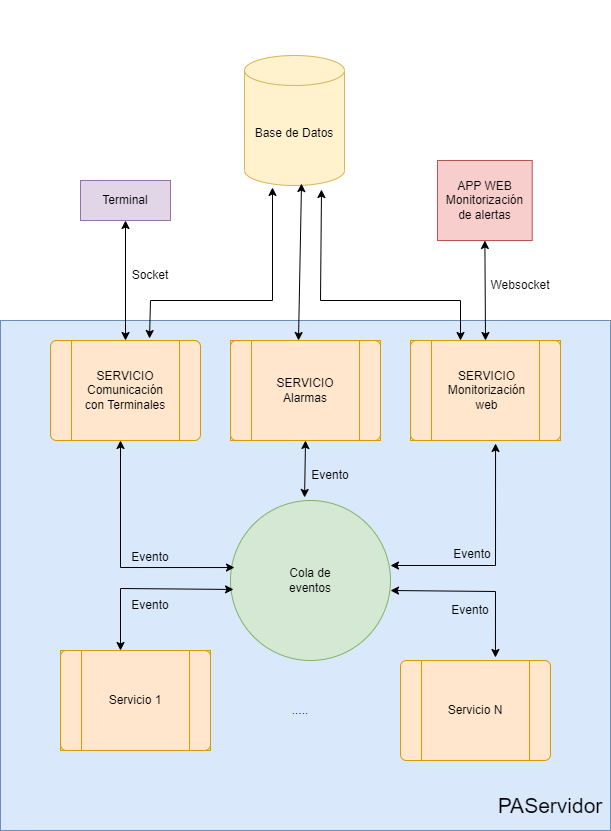
\includegraphics[width=1\textwidth,height=16cm]{Imagenes/Arquitectura-PAServidor}
    \caption{Diagrama arquitectura PAServidor}
    \label{fig:PAServidor}
\end{figure}

Se puede ver el comportamiento de esta arquitectura en el contexto de este proyecto en la \hyperref[subsection-comportamiento]{sección 3.2.1}.

\section{Base de datos}

% Explicar qué partes de la base de datos utilizo de su sistema y con diagramas

Para llevar a cabo el desarrollo, fue proporcionada por parte de la empresa una base de datos de prueba configurada siguiendo el modelo de datos existente de la aplicación de Ibernex.\\

Parte de la información que se tiene que enviar a la web se puede obtener de los eventos que se reciben en el servicio, pero para obtener otros datos es necesario acceder a la base de datos. A continuación se exponen los diagramas de la base de datos utilizados en el contexto de este proyecto.
\begin{itemize}
	\item En la \textit{Figura 2.3} se observa el diagrama de la parte del login y la información de los trabajadores.
	\item En la \textit{Figura 2.4} se observa el diagrama de los pacientes de la institución.
	\item En la \textit{Figura 2.5} se observa el diagrama necesario para procesar las alarmas.
	\item En la \textit{Figura 2.6} se observa el diagrama necesario para procesar las presencias.
\end{itemize}

\begin{figure}[H]
    \centering
    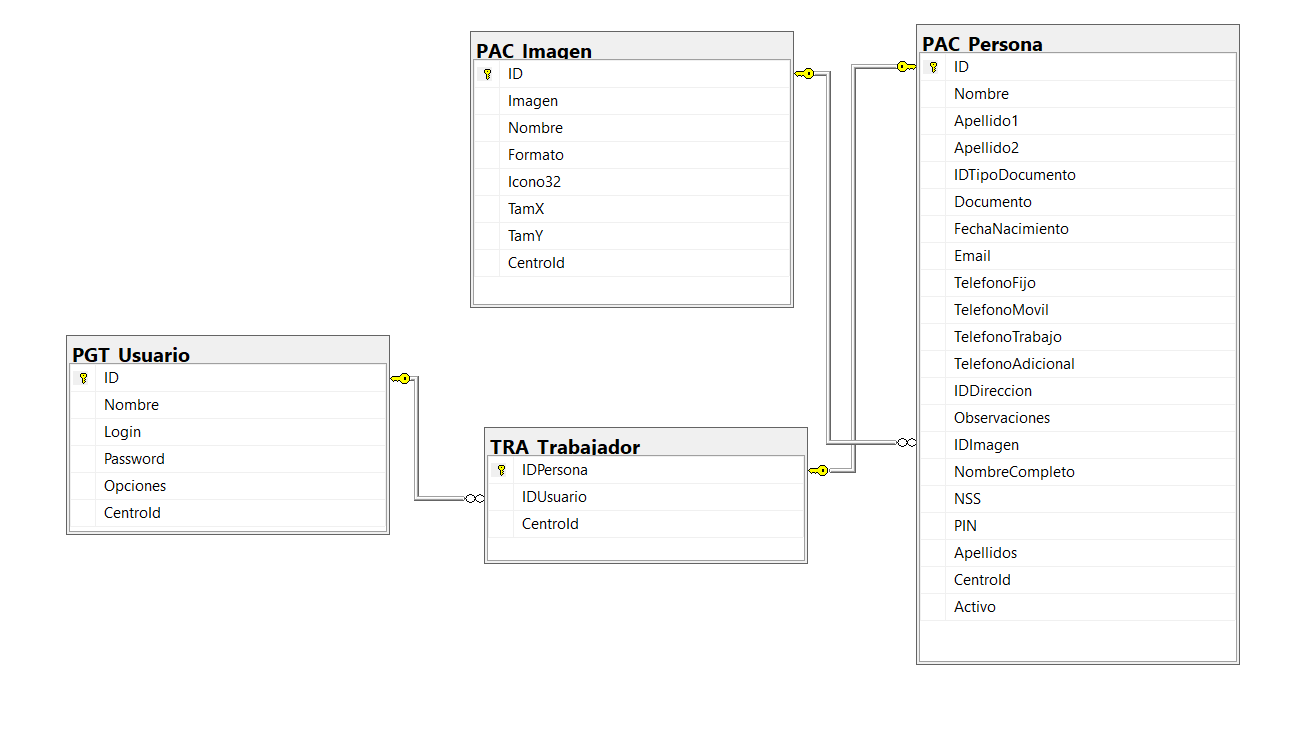
\includegraphics[width=15cm]{Imagenes/Diagrama-BD-Login}
    \caption{Diagrama base de datos - Trabajadores}
    \label{fig:Diagrama-BD-Login}
\end{figure}

\begin{figure}[H]
    \centering
    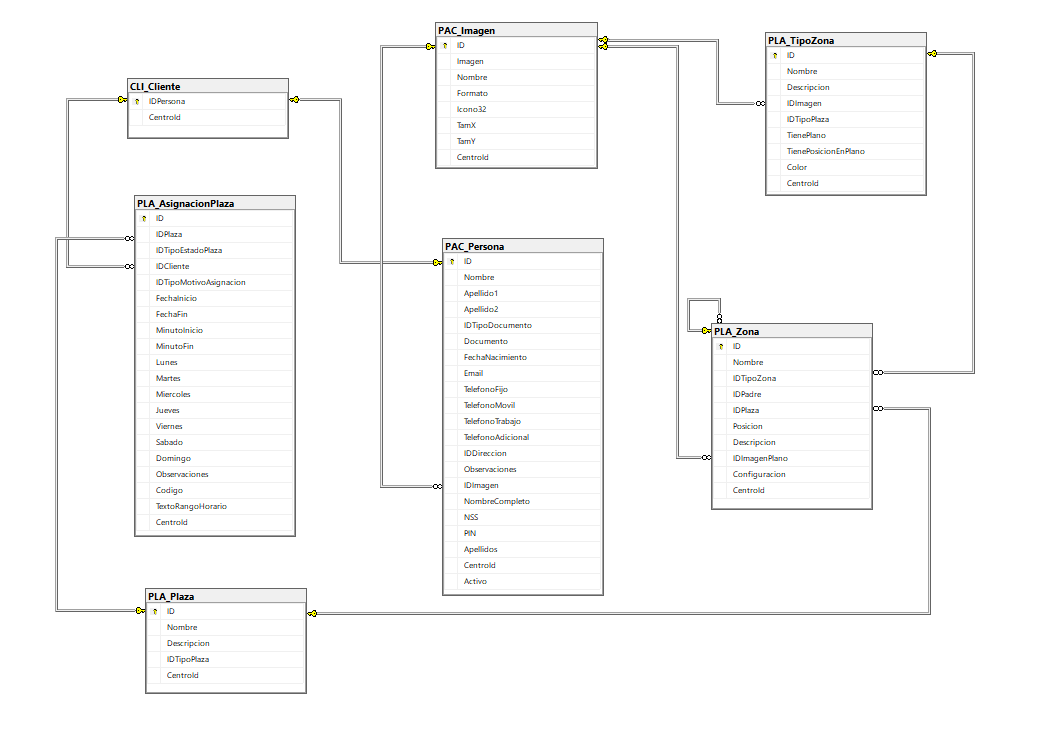
\includegraphics[width=15cm]{Imagenes/Diagrama-BD-Clientes}
    \caption{Diagrama base de datos - Clientes}
    \label{fig:Diagrama-BD-Clientes}
\end{figure}

\begin{figure}[H]
    \centering
    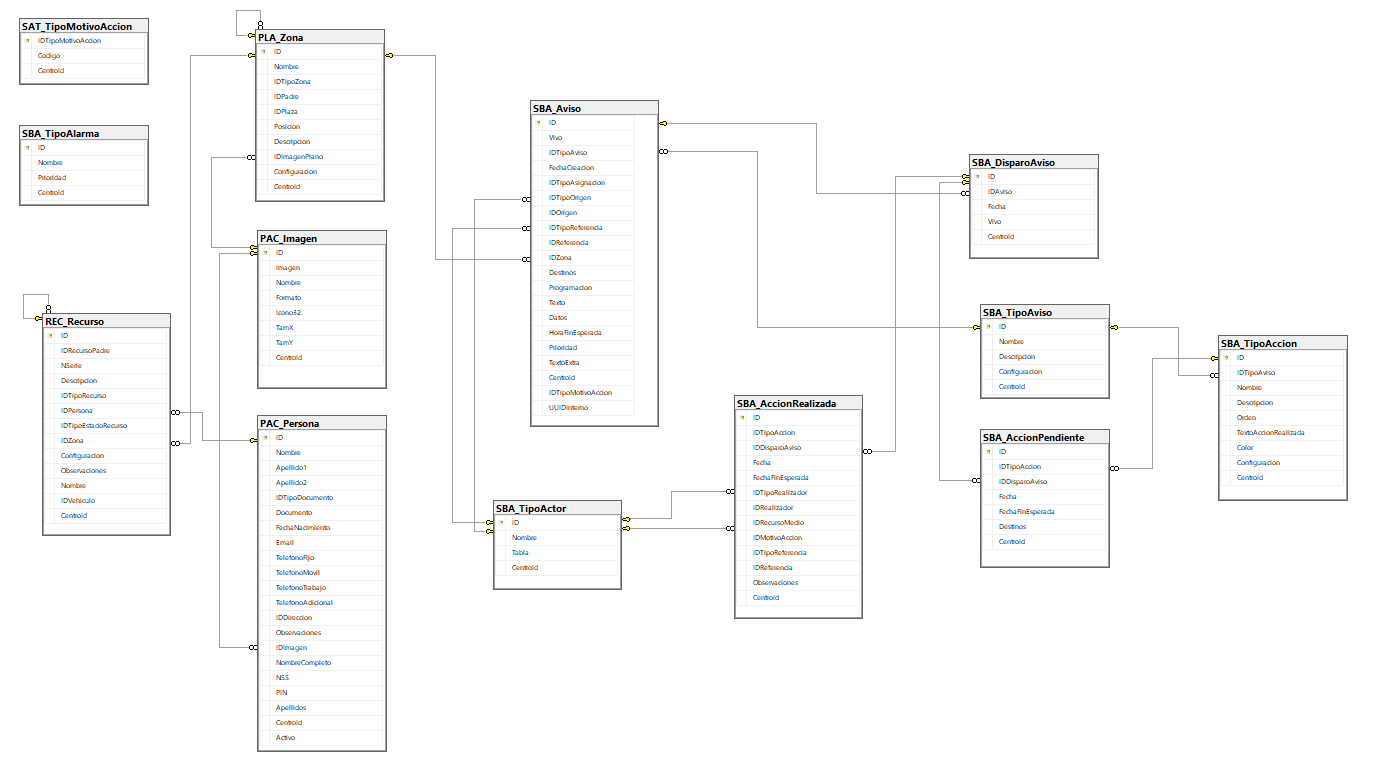
\includegraphics[width=15cm]{Imagenes/Diagrama-BD-Alertas}
    \caption{Diagrama base de datos - Alarmas}
    \label{fig:Diagrama-BD-}
\end{figure}

\begin{figure}[H]
    \centering
    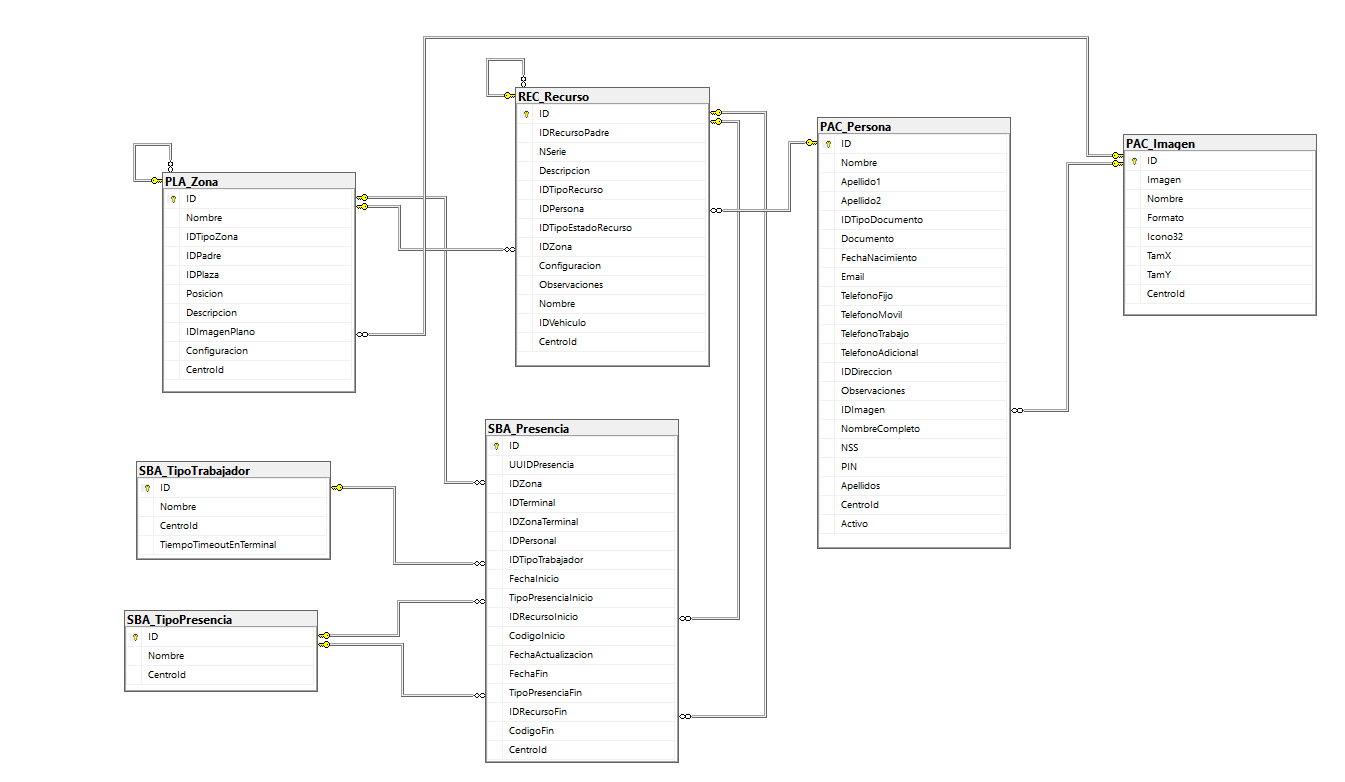
\includegraphics[width=15cm]{Imagenes/Diagrama-BD-Presencias}
    \caption{Diagrama base de datos - Presencias}
    \label{fig:Diagrama-BD-Presencias}
\end{figure}

% INCLUIR EN EL ESQUEMA DEL LOGIN LA TABLA DE LOS RECURSOS DONDE ESTARÁN LOS PUESTOS

% REVISAR EL RESTO DE DIAGRAMAS PARA QUE REALMENTE ESTÉ TODO LO QUE SE HA UTILIZADO

\section{Interfaz de usuario}

% Poner la interfaz final del usuario cuando esté terminada

TODO: Poner la interfaz final del usuario cuando esté terminada

